\section{Results}
\subsection{Resource Usage}
\subsection{Properties}
The sample frequency of the filter is as follows:
\begin{itemize}
\item
Synthesis report
\begin{itemize}
\item Minimum period: 8.653ns
\item Maximum Frequency: 115.571MHz
\end{itemize}
\item
Post-PAR static timing report
\begin{itemize}
\item  Minimum period:   8.711nsns  
\item Maximum frequency: 114.797MHz
\end{itemize}
\end{itemize}
The sample frequency is lower in the static timing report, because it takes into account how the circuit will actually be laid out on the FPGA. The important thing here is that the sample frequency meets the 100 MHz requirement.
\subsection{Analysis of Filter Output }
This section describes the actual effect of the filter on the input audio file. The filter is an upscaler, so besides increasing the sample frequency it should have as little effect as possible on the signal.\\

Figure ~\ref{fig:plot1} shows the audio signal before and after filtering. The filtered signal has a small delay, but its shape is near identical to the original signal. The plot also shows the startup noise of the filter; the first part of the filtered signal is  incorrect. The strength of both signals is about equal, indicating that our filtering coefficients indeed sum up to 1. \\

\begin{figure}
\begin{center}
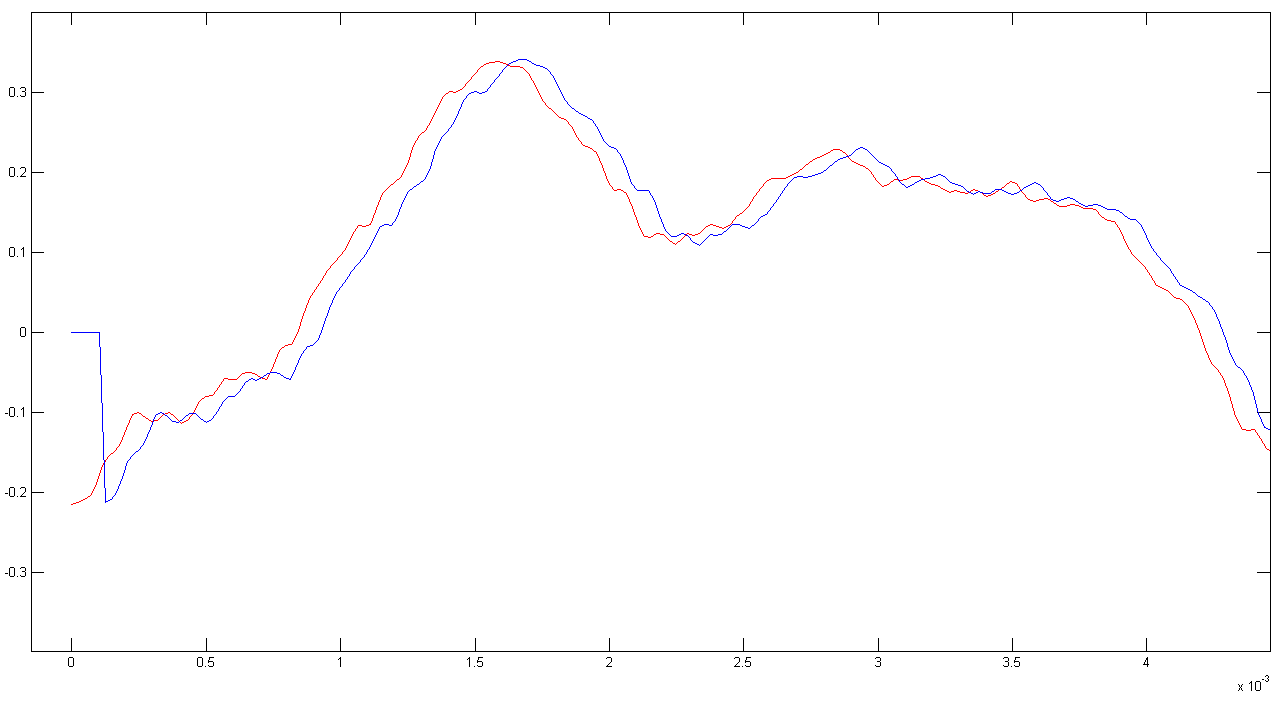
\includegraphics[width=0.7\textwidth]{images/samples3.png}
\caption{Plot of the first part of the original signal (red) and the signal after filtering (blue).}
\label{fig:plot1}
\end{center}
\end{figure}

In figure ~\ref{fig:plot2} we have zoomed in slightly more, shifted the output signal by 4 samples, and drawn dots at the samples. It shows that the sample frequency of the filtered signal is slightly higher than that of the original signal, while their signal values at each time are roughly the same.

\begin{figure}
\begin{center}
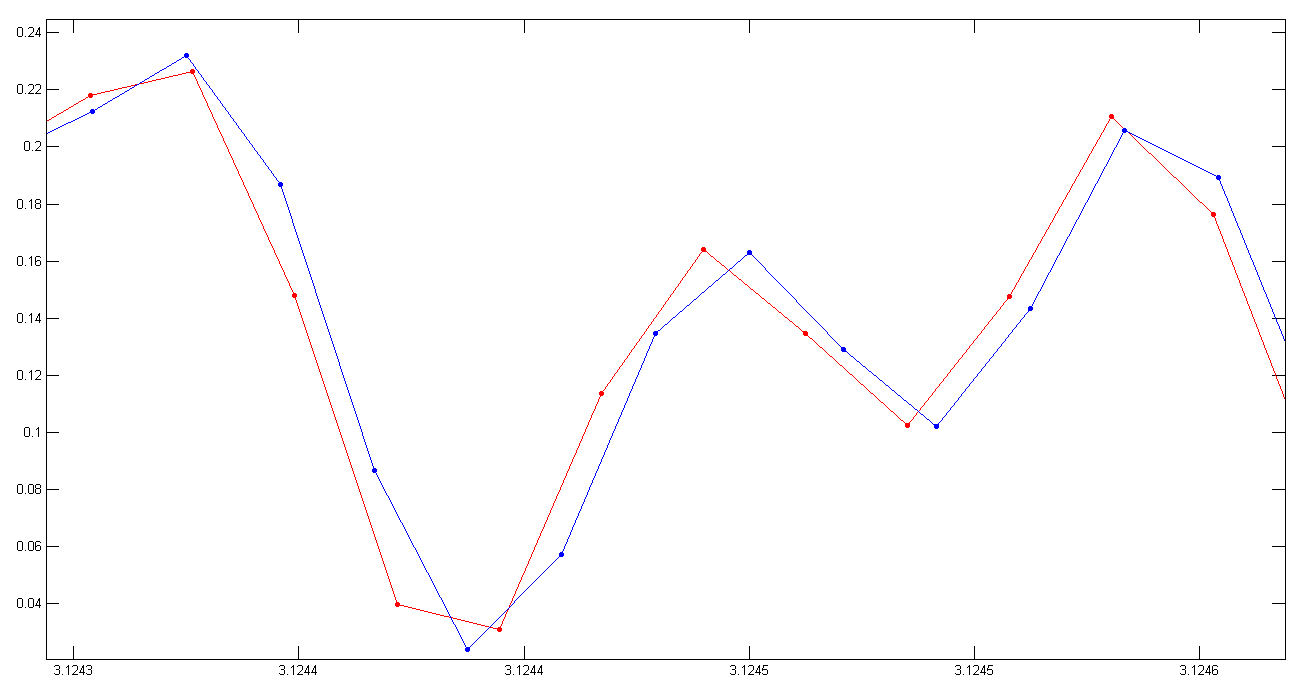
\includegraphics[width=0.7\textwidth]{images/samples.png}
\caption{Plot of part of the original signal (red) and the signal after filtering (blue) with dots indicating the samples.}
\label{fig:plot2}
\end{center}
\end{figure}

Figure ~\ref{fig:spectrum} shows the input and output signal in the frequency domain. There is barely any difference between the two spectra, except for some high frequency harmonics in the output signal. These are explained by the fact that the filtered signal has a higher sample frequency, and therefore the maximum frequency it can represent is higher. But this difference is so small that it does not have any audible effect on the filtered audio.

\begin{figure}
\begin{center}
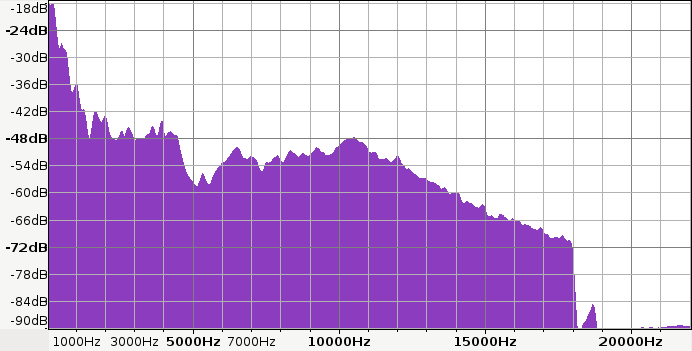
\includegraphics[width=0.7\textwidth]{images/music-input-spectrum.png}
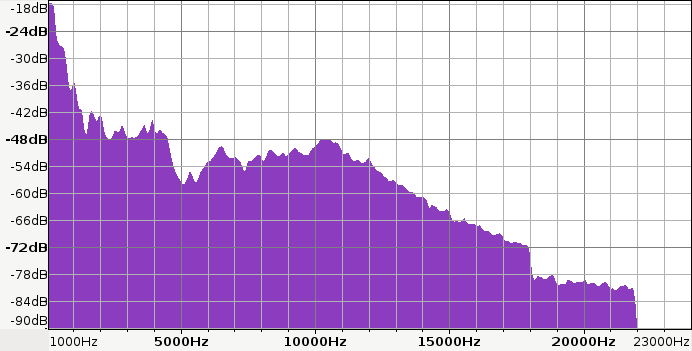
\includegraphics[width=0.7\textwidth]{images/music-output-spectrum.png}
\caption{Plot in the frequency domain of the original signal (top) and the signal after filtering (bottom).}
\label{fig:spectrum}
\end{center}
\end{figure}
